\documentclass[.../main.tex]{subfiles}

\begin{document}

	We start with the two-agent Q-Learning dynamics as presented by Tuyls et al.

	\begin{subequations}
	\label{eqn::EOM}
		\begin{equation}
			\frac{\dot{x}(t)}{x(t)} = \alpha \tau (\sum_{j} a_{ij} y_j - \sum_{i j} x_i a_{ij} y_j)
			+ \alpha \sum_j x_j ln(\frac{x_j}{x_i}) 
		\end{equation}
		\begin{equation}
			\frac{\dot{y}(t)}{y(t)} = \alpha \tau (\sum_{j} b_{ij} x_j - \sum_{i j} y_i b_{ij} x_j)
			+ \alpha \sum_j y_j ln(\frac{y_j}{y_i}).
		\end{equation}
	\end{subequations}

	Here, $\alpha$ and $\tau$ are the parameters of the agent; Sanders et al. refer to these as the memory and intensity of choice parameters respectively. Agent 1 takes action i with probability $x_i$ while Agent 2 takes action j with probability $y_j$. If these actions are taken, the agents receive payoff $a_{ij}$ and $b_{ji}$ respectively. 

	\subsection{Rescaling of Variables} % (fold)
	\label{sub:rescaling_of_variables}
	
		In order to follow the conventions of spin glass
                theory for the analysis of disordered systems, we
                rescale the system so that the payoff matrix elements
                are of order $N^{-1/2}$. The motivation for doing this
                is that, along the way, we will take the limit of the
                number of actions $N$ to infinity. However, doing this
                will result in numerical underflow of the action
                probabilities (i.e. the probability of each action
                goes to zero). To compensate for this, we adjust the
                system so that the sum of the probabilities add to
                $N$. The scaling goes as follows:
%
	\begin{subequations}
		\begin{equation}
			a_{ij} = \sqrt{N} \tilde{a_{ij}}
		\end{equation}
		\begin{equation}
			b_{ji} = \sqrt{N} \tilde{b_{ji}}
		\end{equation}
	\end{subequations}

	We compensate for this change with
	\begin{subequations}
		\begin{equation}
			x_{i} = \tilde{x_{i}}/N
		\end{equation}
		\begin{equation}
			y_{i} = \tilde{y_i}/N.
		\end{equation}
	\end{subequations}

	This gives the original equations as

	\begin{subequations}
	\label{eqn::scaledEOM}
		\begin{equation}
			\frac{\dot{\tilde{x_i}}(t)}{\tilde{x_i}(t)} = \alpha \tilde{\tau} \sum_{j} \tilde{a_
			{ij}} 
			\tilde{y_j} -
			\tilde{\alpha} \tau \frac{1}{\sqrt{N}} \sum_{i j} \tilde{x_i} \tilde{a_{ij}} \tilde{y_j}
			+ \tilde{\alpha} \sum_j \tilde{x_j} ln(\frac{\tilde{x_j}}{\tilde{x_i}}) 
		\end{equation}
		\begin{equation}
			\frac{\dot{\tilde{y_i}}(t)}{\tilde{y_i}(t)} = \alpha \tilde{\tau} \sum_{j} \tilde{b_
			{ij}} 
			\tilde{x_j} -
			\tilde{\alpha} \tau \frac{1}{\sqrt{N}} \sum_{i j} \tilde{y_i} \tilde{b_{ij}} \tilde{x_j}
			+ \tilde{\alpha} \sum_j \tilde{y_j} ln(\frac{\tilde{y_j}}{\tilde{y_i}}).
		\end{equation}
	\end{subequations}

	The need for the factor of $\frac{1}{\sqrt{N}}$ is to follow
        the conventions of the saddle point method of
        integration. This will become clear after taking the
        expectation of the generating functional. Note that we may
        drop the notation on time dependence for $x$ and $y$. However,
        these will always be functions of time. Henceforth, we shall
        not write the tildes on $x, y, a_{ij}, b_{ij}$. We shall also
        abbreviate the final term as
%
	\begin{equation*}
		\rho_{x, i}(t) = \sum_j x_j ln(\frac{x_j}{x_i}) 
	\end{equation*}

	% subsection rescaling_of_variables (end)

	\subsection{Generating Functional} % (fold)
	\label{sub:generating_functional}
	
	The generating functional allows us to take a path integral over all possible realisations of
	learning \cite{SpinGlassTheory}. This is given as:

	\begin{equation}
		Z = \int D[\Vec{x}, \Vec{y}] \prod_i \delta(\textit{equation of motion}_i) exp(i
		\int dt[x_i(t) \psi_i(t) + y_i(t) \phi_i(t)]), 
	\end{equation}

	where the equations of motion are the Lagrange equations of motion given in (
	\ref{eqn::scaledEOM}) andSince
	the fields $\Vec{\psi_i(t)}$ and $\Vec{\phi_i(t)}$ will be set to zero at the end of the
	calculation. $\delta$ denotes the Dirac delta function. We write this in its Fourier
	representation, which yields	

	\begin{equation}
		\begin{split}
	\label{eqn::generatingfunctional}
		Z(\Vec{\psi}, \Vec{\phi}) = \int D[\Vec{x}, \Vec{\hat{x}}, \Vec{y}, \Vec{\hat{y}}] exp(i \sum_i \int dt[\hat{x}_i
		(\frac{\dot{x_i}(t)}{x_i(t)} - \alpha \tilde{\tau} \sum_{j} a_
			{ij} 
			y_j +
			\tilde{\alpha} \tau \frac{1}{\sqrt{N}} \sum_{i j} x_i a_{ij} y_j
			- \tilde{\alpha} \rho_{x, i}(t) + h_{x, i}(t))]) 
			\\
			\times exp(i \sum_i \int dt[\hat{y}_i
		(\frac{\dot{y_i}(t)}{y_i(t)} - \alpha \tilde{\tau} \sum_{j} b_
			{ij} 
			x_j +
			\tilde{\alpha} \tau \frac{1}{\sqrt{N}} \sum_{i j} y_i b_{ij} x_j
			- \tilde{\alpha} \rho_{y, i}(t)+ h_{y, i}(t))])\\
			\times exp(i \sum_i
		\int dt[x_i(t) \psi_i(t) + y_i(t) \phi_i(t))]),
	\end{split}
	\end{equation}

	Here, the terms $a_{ij}, b_{ij}$ are the payoffs in the game and the term $h$ denotes a field
	which will be set to zero at the end of the calculation. We recall that these are randomly
	generated using a multivariate gaussian and then held fixed for the rest of the game. We call
	this 'quenched disorder'. Isolating these terms allows us to rearrange the above as

	\begin{equation}
	\begin{split}
	\label{eqn::moveddisorder}
		Z(\Vec{\psi}, \Vec{\phi}) = \int D[\Vec{x}, \Vec{\hat{x}}, \Vec{y}, \Vec{\hat{y}}] exp(i
		\sum_i \int dt[\hat{x}_i
		(\frac{\dot{x_i}(t)}{x_i(t)}
			- \tilde{\alpha} \rho_{x, i}(t)+ h_{x, i}(t))]) 
			\\
			\times exp(i \sum_i \int dt[\hat{y}_i
		(\frac{\dot{y_i}(t)}{y_i(t)} 
			- \tilde{\alpha} \rho_{y, i}(t) + h_{y, i}(t))])\\
			\times exp(i \sum_i
		\int dt[x_i(t) \psi_i(t) + y_i(t) \phi_i(t))])\\
		\times exp(i \sum_i \int dt[- \hat{x}_i \alpha \tilde{\tau} \sum_{j} a_
			{ij} 
			y_j +
			\hat{x}_i \tilde{\alpha} \tau \frac{1}{\sqrt{N}} \sum_{i j} x_i a_{ij} y_j - \hat{y}_i
			\alpha 
			\tilde{\tau} \sum_{j} b_
			{ij} 
			x_j +
			\hat{y}_i \tilde{\alpha} \tau \frac{1}{\sqrt{N}} \sum_{i j} y_i b_{ij} x_j]).
	\end{split}
	\end{equation}
	The only difference between (\ref{eqn::generatingfunctional}) and (\ref{eqn::moveddisorder}) is
	that we moved the term containing the quenched disorder into a separate exponential. Since our
	aim is to take an average over all possible realisations of this disorder, we will only need to
	focus on the last exponential which we rewrite as

	\begin{equation}
		Q = exp(i \sum_i \int dt[- \hat{x}_i \alpha \tilde{\tau} \sum_{j} a_
			{ij} 
			y_j +
			\hat{x}_i \tilde{\alpha} \tau \frac{1}{\sqrt{N}} \sum_{i j} x_i a_{ij} y_j - \hat{y}_i
			\alpha 
			\tilde{\tau} \sum_{j} b_
			{ij} 
			x_j +
			\hat{y}_i \tilde{\alpha} \tau \frac{1}{\sqrt{N}} \sum_{i j} y_i b_{ij} x_j]).
	\end{equation}

	We will then separate the terms so that like sums are paired together

	\begin{equation}
	\begin{split}
		Q = exp(-i \alpha \tilde{\tau} \sum_{ij} \int dt[\hat{x}_i a_{ij} y_j + \hat{y}_j b_
			{ji} 
			x_i])
			\times
			exp(i \tilde{\alpha} \tau \frac{1}{\sqrt{N}} \sum_{ijk} \int dt[\hat{x}_i x_j
			a_{jk} y_k + \hat{y}_i y_k b_{kj} x_j])
	\end{split}
	\end{equation}

	It should be noted that we have changed some of the subscripts on the terms. Since these terms
	are all multiplied together and we sum over the subscripts, the letters we choose are of no
	importance and we can exchange them freely. We will define both exponentials in $Q$ as $Q_1$ and
	$Q_2$ respectively.

	We are now ready to take the expectation of $Q$. To do this, we will exploit the fact that the
	payoff elements are Gaussian distributed and use the identity \cite{QFTbook}

	\begin{equation}
	\label{eqn::expectationIdentity}
		\int dz [e^{-A_2(z) + \Vec{b} \cdot \Vec{z}}] = (2 \pi)^{k/2} (det(A))^{-1/2} e^{\omega(b)},
	\end{equation}

	where

	\begin{equation*}
		\begin{split}
			A_2(z) = 1/2 \sum_{ij} z_i A_{ij} z_j \\
			\omega_2(z) = 1/2 \sum_{ij} b_i (A)^{-1}_{ij} b_j
		\end{split}
	\end{equation*}

	\subsubsection{Expectation of $Q_1$} % (fold)
	\label{ssub:expectation_of_Q1}
	
	We can rewrite $Q_1$ as 

	\begin{equation*}
		Q_1 = \prod_{ij} exp(\Vec{b} \cdot \Vec{z}),
	\end{equation*}

	where

	\begin{equation*}
		\begin{split}
			b \coloneqq [-i \alpha \tilde{\tau} \int dt[\hat{x}_i y_j], -i \alpha \tilde{\tau} \int
			dt[\hat{y}_j x_i]]^T \\
			z \coloneqq [a_{ij}, b_{ji}]^T\\
			A \coloneqq \Sigma^{-1}\\
			\Sigma_{ij} \coloneqq Cov[z_i, z_j],
		\end{split}
	\end{equation*}

	where $\Sigma$ is the covariance of $\Vec{z}$. We recall that the scaled system has
	payoff elements chosen so that

	\begin{equation*}
		\begin{split}
			\mathbb{E}[a_{ij}] = \mathbb{E}[b_{ji}] = 0\\
			\mathbb{E}[a_{ij}^2] = \mathbb{E}[b_{ji}^2] = 1/N\\
			\mathbb{E}[a_{ij} b_{ji}] = \Gamma /N.
		\end{split}
	\end{equation*}

	Applying identity (\ref{eqn::expectationIdentity}) gives:

	\begin{equation}
	\begin{split}
		\mathbb{E}[Q_1] = \prod_{ij} exp(- \alpha^2 \tilde{\tau}^2 \frac{1}{2N} \int dt dt'[
		\hat{x}_i
		(t) \hat{x}_i
		(t') y_j(t) y_j(t') + \hat{y}_j(t) \hat{y_j}(t') x_i(t) x_i(t') \\ + \Gamma \hat{x}_i(t) 
		{x}_i
		(t') {y}_j(t) \hat{y}_j(t') + \Gamma \hat{y}_j(t) {y}_j(t') {x}_i(t) \hat{x}_i(t')]).
	\end{split}
	\end{equation}

	% subsubsection expectation_of_Q1 (end)
	% subsection generating_functional (end)

	\subsubsection{Expectation of $Q_2$} % (fold)
	\label{ssub:expectation_of_Q2}
	
	We take a similar approach with the following definitions

	\begin{equation*}
		\begin{split}
			b \coloneqq [i \tilde{\alpha} \tau \int dt[\hat{x}_i x_j y_k], i \tilde{\alpha} 
			\tau
			\int
			dt[\hat{y}_i x_j y_k]]^T \\
			z \coloneqq [a_{jk}, b_{kj}]^T\\
			A \coloneqq \Sigma^{-1}\\
			\Sigma_{ij} \coloneqq Cov[z_i, z_j],
		\end{split}
	\end{equation*}

	% subsubsection expectation_of_Q2 (end)

	Following the same procedure as for $Q_1$ yields

	\begin{equation}
	\begin{split}
		\mathbb{E}[Q_2] = \prod_{ij} exp(- \tilde{\alpha}^2 \tau^2 \frac{1}{2N^2} \int dt dt'[
		\hat{x}_i
		(t) \hat{x}_i
		(t') x_j(t) x_j(t') y_k(t) y_k(t') \\+ \hat{y}_i(t) \hat{y_i}(t') x_j(t) x_j(t') y_k(t)
		y_k(t') \\ + \Gamma \hat{x}_i(t) \hat{y}_i(t')
		{x}_j
		(t) x_j{(t')} {y}_k(t) y_k(t') \\ + \Gamma \hat{y}_i(t) \hat{x}_i(t') {x}_j(t) {x}_j(t')
		y_k(t) y_k(t')]).
	\end{split}
	\end{equation}


	We now define the correlation functions

		\begin{align*}
C_x(t, t') &= N^{-1} \sum_i x_i(t) x_i(t') & C_y(t, t') &= N^{-1} \sum_i y_i(t) y_i(t')\\
L_x(t, t') &= N^{-1} \sum_i \hat{x}_i(t) \hat{x}_i(t') & L_y(t, t') &= N^{-1} \sum_i \hat{y}_i(t) \hat{y}_i(t') \\
K_x(t, t') &= N^{-1} \sum_i x_i(t) \hat{x}_i(t') & K_y(t, t') &= N^{-1} \sum_i y_i(t) \hat{y}_i(t')\\
A_{xy}(t, t') &= N^{-1} \sum_i \hat{x}_i(t) \hat{y}_i(t').
\end{align*}
	% section derivation (end)

We then rewrite $\mathbb{E}[Q]$ as 

\begin{equation}
\begin{split}
		\mathbb{E}[Q] = exp(- \alpha^2 \tilde{\tau}^2 \frac{N}{2} \int dt dt'[L_x(t, t')C_y(t, t')
		+ L_y(t, t')C_x(t, t') + 2 \Gamma K_x(t, t') K_y(t', t)] \\
	- \tilde{\alpha}^2 \tau^2 \frac{N}{2} \int dtdt' [L_x(t, t') C_x(t, t') C_y(t, t') + L_y(t, t')
	C_x(t, t') C_y(t, t') \\ + \Gamma A_{xy}(t, t') C_x(t, t') C_y(t, t') + \Gamma A_{xy}(t', t) C_x
	(t, t') C_y(t, t')] )
\end{split}
\end{equation}

We can introduce these correlation functions into the expectation which gives

\begin{equation}
	\begin{split}
		\mathbb{E}[Q] = \int D[C_x, \hat{C_x}, L_x, \hat{L_x}, K_x, 
		\hat{K_x}, C_y, \hat{C_y}, L_y, \hat{L_y}, K_y, 
		\hat{K_y}, A_{xy}, \hat{A}_{xy}] 
		exp(N(\Psi, \Phi, \Lambda)),
	\end{split}
\end{equation}

where
\begin{equation}
	\begin{split}
	\Psi = i \int dtdt' [\hat{C}_x(t, t') C_x(t, t') + \hat{L}_x(t, t') L_x(t, t') + \hat{K}_x
		(t, t') K_x(t, t') \\ + \hat{C}_y(t, t') C_y(t, t') + \hat{L}_y(t, t') L_y(t, t') + 
		\hat{K}_y(t, t') K_y(t, t') + \hat{A}_{xy}(t, t') A_{xy}(t, t')]
	\end{split}
\end{equation}

\begin{equation}
	\begin{split}
		\Phi = - \alpha^2 \tilde{\tau}^2 \frac{N}{2} \int dt dt'[L_x(t, t')C_y(t, t')
		+ L_y(t, t')C_x(t, t') + 2 \Gamma K_x(t, t') K_y(t', t)] \\
	- \tilde{\alpha}^2 \tau^2 \frac{N}{2} \int dtdt' [L_x(t, t') C_x(t, t') C_y(t, t') + L_y(t, t')
	C_x(t, t') C_y(t, t') \\ + \Gamma A_{xy}(t, t') C_x(t, t') C_y(t, t') + \Gamma A_{xy}(t', t) C_x
	(t, t') C_y(t, t')] 
\end{split}
\end{equation}

\begin{equation}
	\begin{split}
		\Lambda = i \sum_i \int dt dt'[\hat{C}_x(t, t') x_i(t) x_i(t') + \hat{L}_x(t, t') \hat{x}_i
		(t)\hat{x}_i(t') + \hat{K}_x(t, t') x_i(t) \hat{x}_i(t') \\ + \hat{C}_y(t, t') y_i(t) y_i
		(t') +
		\hat{L}_y(t, t') \hat{y}_i
		(t)\hat{y}_i(t') + \hat{K}_y(t, t') y_i(t) \hat{y}_i(t') \\ 
		+ \hat{A}_{xy}(t, t') \hat{x}_i(t) \hat{y}_i(t')].
	\end{split}
\end{equation}

We insert this expectation back into the original generating functional which gives

\begin{equation}
	\begin{split}
		\mathbb{E}[Z(\Vec{\psi}, \Vec{\phi})] = \int D[C_x, \hat{C_x}, L_x, \hat{L_x}, K_x, 
		\hat{K_x}, C_y, \hat{C_y}, L_y, \hat{L_y}, K_y, 
		\hat{K_y}, A_{xy}, \hat{A}_{xy}] 
		exp(N(\Psi, \Phi, \Omega + (\mathcal{O}(N^{-1})))),
	\end{split}
\end{equation}

where $\Omega$ includes all terms describing the time evolution of the system and is given by

\begin{equation}
	\begin{split}
		\Omega = N^{-1} \sum_i log \int D[x_i, \hat{x}_i, y_i, \hat{y}_i] exp(i
		\int dt[\hat{x}_i
		(\frac{\dot{x_i}(t)}{x_i(t)}
			- \tilde{\alpha} \rho_{x, i}(t) + h_{x, i}(t))]) 
			\\
		\times exp(i\int dt dt'[\hat{C}_x(t, t') x_i(t) x_i(t') + \hat{L}_x(t, t') \hat{x}_i
		(t)\hat{x}_i(t') + \hat{K}_x(t, t') x_i(t) \hat{x}_i(t')])\\
		\times exp(i \int dt[\hat{y}_i
		(\frac{\dot{y_i}(t)}{y_i(t)} 
			- \tilde{\alpha} \rho_{y, i}(t) + h_{y, i}(t))])\\
		\times exp(i \int dt dt' [\hat{C}_y(t, t') y_i(t) y_i
		(t') +
		\hat{L}_y(t, t') \hat{y}_i
		(t)\hat{y}_i(t') + \hat{K}_y(t, t') y_i(t) \hat{y}_i(t')])\\
		\times exp(i \int dt dt'[\hat{A}_{xy}(t, t') \hat{x}_i(t) \hat{y}_i(t')]])
			\times exp(i \sum_i
		\int dt[x_i(t) \psi_i(t) + y_i(t) \phi_i(t))]).
	\end{split}
\end{equation}

We will evaluate the path integral using the saddle point method for integration 
\cite{saddlepoint}. In this method, we consider that the integration is dominated by the maximum of
the function 

\begin{equation*}
	f = \Psi + \Phi + \Omega,
\end{equation*}

and we take the limit as N extends to infinity. We therefore determine the relations which maximise
this function. We find

\begin{align*}
	\frac{\partial f}{\partial C_x(t, t')} &\implies i \hat{C}_x(t, t') = \frac{\alpha^2 
	\tilde{\tau}^2}{2} L_y(t, t') + \frac{\tilde{\alpha}^2 \tau^2}{2}(L_x(t, t')C_y(t, t') + L_y
	(t, t')C_y(t, t') + 2\Gamma A_{xy}(t, t') C_y(t, t'))\\
	\frac{\partial f}{\partial L_x(t, t')} &\implies i \hat{L}_x(t, t') = \frac{\alpha^2 
	\tilde{\tau}^2}{2} C_y(t, t') + \frac{\tilde{\alpha}^2 \tau^2}{2}(C_x(t, t') C_y(t, t'))\\
	\frac{\partial f}{\partial K_x(t, t')} &\implies i\hat{K}_x(t, t') = \alpha^2 
	\tilde{\tau}^2 \Gamma K_y(t', t) \\
	\frac{\partial f}{\partial C_y(t, t')} &\implies i \hat{C}_y(t, t') = \frac{\alpha^2 
	\tilde{\tau}^2}{2} L_x(t, t') + \frac{\tilde{\alpha}^2 \tau^2}{2}(L_x(t, t')C_x(t, t') + L_y
	(t, t')C_x(t, t') + 2\Gamma A_{xy}(t, t') C_x(t, t'))\\
	\frac{\partial f}{\partial L_y(t, t')} &\implies i \hat{L}_y(t, t') = \frac{\alpha^2 
	\tilde{\tau}^2}{2} C_x(t, t') + \frac{\tilde{\alpha}^2 \tau^2}{2}(C_x(t, t') C_y(t, t'))\\
	\frac{\partial f}{\partial K_y(t, t')} &\implies i\hat{K}_y(t, t') = \alpha^2 
	\tilde{\tau}^2 \Gamma K_x(t', t) \\
	\frac{\partial f}{\partial A_{xy}(t, t')} &\implies i\hat{A}_{xy}(t, t') = \tilde{\alpha}^2
	\tau^2 \Gamma C_x(t, t') C_y(t, t').
\end{align*}

Similarly,

\begin{align*}
	\frac{\partial f}{\partial \hat{C}_x(t, t')} &\implies C_x(t, t') = \lim_{N \rightarrow \infty}
N^{-1} \sum_i \langle x_i(t) x_i(t')\rangle _\Omega = -\lim_{N \rightarrow \infty} \sum_i
\frac{\partial^2\mathbb{E}[Z(\psi, \phi)]}{\partial \psi_i(t) \partial \psi_i (t')} \bigg|_{\Vec
{\phi} = \Vec{\psi} = \Vec{h} = 0}\\
	\frac{\partial f}{\partial \hat{L}_x(t, t')} &\implies L_x(t, t') = \lim_{N \rightarrow \infty}
N^{-1} \sum_i \langle \hat{x}_i(t) \hat{x}_i(t')\rangle _\Omega = -\lim_{N \rightarrow \infty} \sum_i
\frac{\partial^2\mathbb{E}[Z(\psi, \phi)]}{\partial h_{x,i}(t) \partial h_{x, i} (t')} \bigg|_{\Vec
{\phi} = \Vec{\psi} = \Vec{h} = 0}\\
	\frac{\partial f}{\partial \hat{K}_x(t, t')} &\implies K_x(t, t') = \lim_{N \rightarrow \infty}
N^{-1} \sum_i \langle x_i(t) \hat{x}_i(t')\rangle _\Omega = -\lim_{N \rightarrow \infty} \sum_i
\frac{\partial^2\mathbb{E}[Z(\psi, \phi)]}{\partial \Vec{\psi}(t) \partial h_{x, i} (t')}
\bigg|_{\Vec{\phi} = \Vec{\psi} = \Vec{h} = 0}\\
\frac{\partial f}{\partial \hat{C}_y(t, t')} &\implies C_y(t, t') = \lim_{N \rightarrow \infty}
N^{-1} \sum_i \langle y_i(t) y_i(t')\rangle _\Omega = -\lim_{N \rightarrow \infty} \sum_i
\frac{\partial^2\mathbb{E}[Z(\psi, \phi)]}{\partial \phi_i(t) \partial \phi_i (t')} \bigg|_{\Vec
{\phi} = \Vec{\psi} = \Vec{h} = 0}\\
	\frac{\partial f}{\partial \hat{L}_y(t, t')} &\implies L_y(t, t') = \lim_{N \rightarrow \infty}
N^{-1} \sum_i \langle \hat{y}_i(t) \hat{y}_i(t')\rangle _\Omega = -\lim_{N \rightarrow \infty} \sum_i
\frac{\partial^2\mathbb{E}[Z(\psi, \phi)]}{\partial h_{y,i}(t) \partial h_{y, i} (t')} \bigg|_{\Vec
{\phi} = \Vec{\psi} = \Vec{h} = 0}\\
	\frac{\partial f}{\partial \hat{K}_y(t, t')} &\implies K_y(t, t') = \lim_{N \rightarrow \infty}
N^{-1} \sum_i \langle y_i(t) \hat{y}_i(t')\rangle _\Omega = -\lim_{N \rightarrow \infty} \sum_i
\frac{\partial^2\mathbb{E}[Z(\psi, \phi)]}{\partial \Vec{\phi}(t) \partial h_{x, i} (t')}
\bigg|_{\Vec{\phi} = \Vec{\psi} = \Vec{h} = 0}\\
	\frac{\partial f}{\partial \hat{A}_{xy}(t, t')} &\implies A_{xy}(t, t') = \lim_{N \rightarrow
	\infty}
N^{-1} \sum_i \langle \hat{x}_i(t) \hat{y}_i(t')\rangle _\Omega = -\lim_{N \rightarrow \infty} \sum_i
\frac{\partial^2\mathbb{E}[Z(\psi, \phi)]}{\partial \partial h_{x, i} (t) \partial h_{y, i} (t')}
\bigg|_{\Vec{\phi} = \Vec{\psi} = \Vec{h} = 0}.\\
\end{align*}

We implement these relations into the expression of $\Omega$, and make the assumption that all
actions $i$ are independent and identically distributed (i.i.d.), which gives

\begin{equation}
	\begin{split}
		\Omega =log \int D[x, \hat{x}, y, \hat{y}] exp(i
		\int dt[\hat{x}(t)
		(\frac{\dot{x}(t)}{x(t)}
			- \tilde{\alpha} \rho_{x}(t))]) 
			\\
		\times exp(-\int dt dt'[\frac{1}{2} \alpha^2 \tilde{\tau}^2 C_y(t, t')\hat{x}(t)\hat{x}(t')
		+ \frac{1}{2} \tilde{\alpha}^2 \tau^2 C_x(t, t')C_y(t, t')\hat{x}(t)\hat{x}(t') + i \alpha^2
		\tilde{\tau}^2 \Gamma G_y(t', t) x(t) \hat{x}(t')])\\
		\times exp(i \int dt[\hat{y}(t)
		(\frac{\dot{y}(t)}{y(t)} - \tilde{\alpha} \rho_{y}(t))])\\
		\times exp(-\int dt dt'[\frac{1}{2} \alpha^2 \tilde{\tau}^2 C_x(t, t')\hat{y}(t)\hat{y}(t')
		+ \frac{1}{2} \tilde{\alpha}^2 \tau^2 C_x(t, t')C_y(t, t')\hat{y}(t)\hat{y}(t') + i \alpha^2
		\tilde{\tau}^2 \Gamma G_x(t, t') y(t) \hat{y}(t')])\\
		\times exp(-\int dt dt'[\tilde{\alpha}^2 \tau^2 \Gamma C_x(t, t') C_y(t, t') \hat{x}(t) 
		\hat{y}
		(t')]).
	\end{split}
\end{equation}

Since this contains all of the information of the learning evolution, we consider $\Omega$ as an
effective generating functional (and in fact we see that it has a similar structure to (
\ref{sub:generating_functional}), without the existence of the fields $\psi, \phi$). In particular
we recognise this as the generating functional of the 'effective dynamics' given as

\begin{equation}
	\begin{split}
		\dot{x}(t) &= x(t)(\Gamma \alpha^2 \tilde{\tau}^2 \int dt'[G_y(t, t')x(t')] + 
		\tilde{\alpha}
		\rho_x(t) + \alpha \tilde{\tau} \eta_x(t) + \tilde{\alpha} \tau \eta_x(t) \eta_y(t) +
		\sqrt{\Gamma} \tilde{\alpha} \tau \mu_x) \\
		\dot{y}(t) &= y(t)(\Gamma \alpha^2 \tilde{\tau}^2 \int dt'[G_x(t, t')y(t')] + 
		\tilde{\alpha} \rho_y(t) +
		\alpha \tilde{\tau} \eta_y(t) + \tilde{\alpha} \tau \eta_x(t) \eta_y(t)+ 
		\sqrt{\Gamma} \tilde{\alpha} \tau \mu_y), \\
	\end{split}
\end{equation}

with the self-consistency relations

\begin{align}
	G_x(t, t') &= \langle \frac{\delta x(t)}{\delta \eta_x(t')}\rangle  & G_y(t, t') &= \langle \frac{\delta y(t)}{\delta
	\eta_y(t')}\rangle  \\
	\langle \eta_x(t) \eta_x(t')\rangle  &= C_y(t, t') & \langle \eta_y(t) \eta_y(t')\rangle  &= C_x(t, t')\\
	\langle \mu_x(t) \mu_y(t')\rangle  &= C_x(t, t') C_y(t, t') & \langle \mu_x(t) \mu_x(t')\rangle  &= \langle \mu_y(t) \mu_y(t')\rangle  = 0
\end{align}

\section{Stability Analysis} % (fold)
\label{sec:stability_analysis}

We are now in a position to take the effective dynamics, which describes the evolution of the
learning dynamics after averaging over all possible realisations of the payoff elements, and
determine the stability of the system at fixed points. We will follow the procedure laid out by
Opper et al \cite{Opper}. First, we rewrite $x(t)$, $y(t)$ as perturbations about their fixed
points. We will then analyse the stability of these fixed points.

Let

\begin{align}
	x(t) = x^* + \hat{x}(t) \\
	y(t) = y^* + \hat{y}(t) \\
	\eta_x(t) = \eta_x^* + \hat{\nu}_x(t)\\
	\eta_y(t) = \eta_y^* + \hat{\nu}_y(t)\\
	\mu_x(t) = \mu_x^* + \hat{\delta}_x(t)\\
	\mu_y(t) = \mu_y^* + \hat{\delta}_y(t),
\end{align}

where terms denoted by $\cdot^*$ are the values that are taken at the fixed point and terms denoted
by $\hat{\cdot}$ refer to deviations from the fixed point. This is not to be confused with
the conjugate variable notation that we used in the previous section. We assume that these
perturbations arise from additive noise, $\xi(t)$, $\zeta(t)$, drawn from the unit normal
distribution which are applied to the dynamics. Rewriting the dynamics with all of these
considerations gives

\begin{equation}
	\begin{split}
		\frac{d}{dt} (x^* + \hat{x}(t)) = (x^* + \hat{x}(t))(\Gamma \alpha^2 \tilde{\tau}^2 \int dt'
		[G_y(t, t')(x^* + \hat{x}(t'))] + \tilde{\alpha} \rho_x(t) + \alpha \tilde{\tau} (\eta_x^* + \hat{\nu}_x
		(t)) \\ + \tilde{\alpha} \tau (\eta_x^* + \hat{\nu}_x(t)) (\eta_y^* + \hat{\nu}_y(t)) + \sqrt{\Gamma} \tilde{\alpha} \tau (\mu_x^* + \hat{\delta}_x(t)) + \xi(t)) \\
		\frac{d}{dt} (y^* + \hat{y}(t)) = (y^* + \hat{y}(t))(\Gamma \alpha^2 \tilde{\tau}^2 \int dt'
		[G_x(t, t')(y^* + \hat{y}(t'))] + \tilde{\alpha} \rho_y(t) + \alpha \tilde{\tau} (\eta_y^* + \hat{\nu}_y
		(t)) \\ + \tilde{\alpha} \tau (\eta_x^* + \hat{\nu}_x(t)) (\eta_y^* + \hat{\nu}_y(t))
		 + \sqrt{\Gamma} \tilde{\alpha} \tau (\mu_y^* + \hat{\delta}_y(t)) + \zeta(t)).
	\end{split}
\end{equation}

Considering only terms which are linear in the deviations yields

\begin{equation} 
	\label{eqn::Linearisation}
	\begin{split}
	\frac{d}{dt} \hat{x}(t) = (x^* + \hat{x}(t))\left[ \Gamma \alpha^2 \tilde{\tau}^2 x^* \int G_y(t - t') dt' + \tilde{\alpha} \rho_x^* + \alpha \tilde{\tau} \eta_x^* + \tilde{\alpha} \tau \eta_x^* \eta_y^* + \Gamma \tilde{\alpha} \tau \mu_x \right] \\
	+ x^* \left[ \Gamma \alpha^2 \tilde{\tau}^2 \int G_y(t - t') \hat{x}(t') dt' + \alpha \tilde{\tau} \hat{\nu}_x(t) + \tilde{\alpha} \tau \eta_x^* \hat{\nu}_y(t) + \tilde{\alpha} \tau \eta_y^* \hat{\nu}_x(t) + \sqrt{\Gamma} \tilde{\alpha} \tau \hat{\delta}_x(t) + \xi(t) \right]\\
	\frac{d}{dt} \hat{y}(t) = (y^* + \hat{y}(t))\left[ \Gamma \alpha^2 \tilde{\tau}^2 x^* \int G_x(t - t') dt' + \tilde{\alpha} \rho_y^* + \alpha \tilde{\tau} \eta_y^* + \tilde{\alpha} \tau \eta_x^* \eta_y^* + \Gamma \tilde{\alpha} \tau \mu_y \right] \\
	+ y^* \left[ \Gamma \alpha^2 \tilde{\tau}^2 \int G_x(t - t') \hat{y}(t') dt' + \alpha \tilde{\tau} \hat{\nu}_y(t) + \tilde{\alpha} \tau \eta_x^* \hat{\nu}_y(t) + \tilde{\alpha} \tau \eta_y^* \hat{\nu}_x(t) + \sqrt{\Gamma} \tilde{\alpha} \tau \hat{\delta}_y(t) + \zeta(t) \right].\\
	\end{split}
\end{equation}


If we consider the long term behaviour of the system near a stable fixed point, then $\hat{x}(t)$ goes to zero as $t \rightarrow \infty$. This yields the requirement that a fixed point $x^*$ must satisfy


\begin{equation}
	0 = x^* \left[\Gamma \alpha^2 \tilde{\tau}^2 x^* \int G_y(t - t') dt' + \tilde{\alpha} \rho_x^* + \alpha \tilde{\tau} \eta_x^* + \tilde{\alpha} \tau \eta_x^* \eta_y^* + \sqrt{\Gamma} \tilde{\alpha} \tau \mu_x \right].
\end{equation}

The implication here is that the resulting value of $x^*$ can take two solutions. However, one of these is $x^* = 0$, which is found to rarely occur, while the second solution contains a term $\sqrt{\Gamma}$, which would yield complex values. If this is true, then it would imply that the learning algorithm will rarely converge for values of $\Gamma < 0$. Numerical experiments will shed more light on the likelihood of convergence. If this ansatz turns out to be incorrect (i.e. we see significant convergence for $\Gamma < 0$), it is unlikely that we will be able to solve for the stability line for this case.  

We continue to follow the method of Opper et al. by taking the Fourier transform of (\ref{eqn::Linearisation}). For both agents, the first term in square brackets is constant with respect to time and so will not affect the long term behaviour of the system. We can, therefore, ignore this and focus on the second term. For the sake of brevity, we will only write the equations for Agent 1 (i.e. for $x$), though the equations for y can be equivalently obtained. Taking the Fourier transform yields

\begin{equation}
	\left[ \frac{i \omega}{x^*} - \Gamma \alpha^2 \tilde{\tau}^2 \mathcal{G}_y(\omega)\right] \mathcal{X}(w) = \Gamma \alpha \tilde{\tau} \mathcal{V}_x(\omega) + \tilde{\alpha} \tau \eta^*_x \mathcal{V}_y(\omega) + \tilde{\alpha} \tau \eta^*_y \mathcal{V}_x(\omega) + \sqrt{\Gamma} \tilde{\alpha} \tau \Delta(\omega) + \Xi(\omega).
\end{equation} 

Then,

\begin{equation} \label{eqn::Transformed}
	\left<[|\mathcal{X}(\omega)|^2 \right> = \left< | \Gamma \alpha \tilde{\tau} \mathcal{V}_x(\omega) + \tilde{\alpha} \tau \eta^*_x \mathcal{V}_y(\omega) + \tilde{\alpha} \tau \eta^*_y \mathcal{V}_x(\omega) + \sqrt{\Gamma} \tilde{\alpha} \tau \Delta(\omega) + \Xi(\omega) |^2 \right> \frac{1}{\left< |\mathcal{A}(\omega, x^*) |^2 \right>}, 
\end{equation}


where

\begin{equation}
	\mathcal{A}(\omega, x^*) = \frac{i \omega}{x^*} - \Gamma \alpha^2 \tilde{\tau}^2 \mathcal{G}_y(\omega)
\end{equation}

The behaviour of this line for $\omega = 0$ gives the long term behaviour of the system. By
considering that, for a stable fixed point to exist, $\left<[|\mathcal{X}(\omega = 0)|^2 \right>$,
we arrive at an expression for a stability line (i.e. the phase transition between the existence of
stable fixed points and unstable behaviour).


% section stability_analysis (end)

\section{Numerical Simulations} % (fold)
\label{sec:numerical_simulations}

\begin{figure}[h]
	\centering
	\begin{subfigure}[b]{0.45 \textwidth}
	\centering
	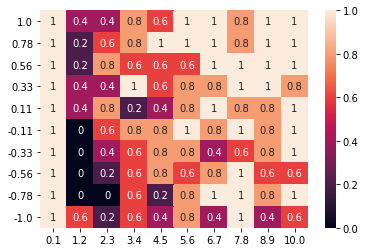
\includegraphics[width = 0.7 \textwidth]{Figures/Run1.png}
	\caption{$\alpha = 0.1$}
	\end{subfigure}
	\begin{subfigure}[b]{0.45 \textwidth}
	\centering
	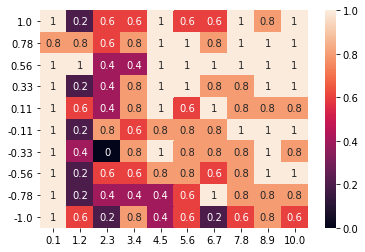
\includegraphics[width = 0.7 \textwidth]{Figures/Run2.png}
	\caption{$\alpha = 0.1$}
	\end{subfigure}
	%
	\begin{subfigure}[b]{0.45 \textwidth}
	\centering
	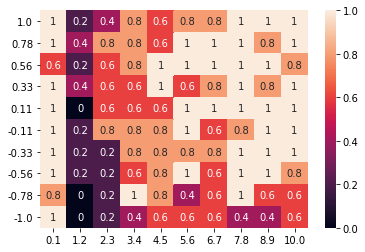
\includegraphics[width = 0.7 \textwidth]{Figures/Alpha_2.png}
	\caption{$\alpha = 0.2$}
	\end{subfigure}
	\begin{subfigure}[b]{0.45 \textwidth}
	\centering
	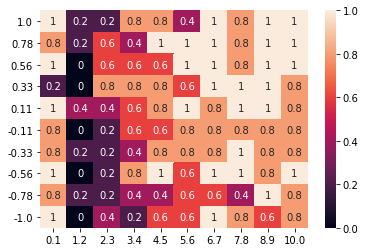
\includegraphics[width = 0.7 \textwidth]{Figures/Alpha_2_Run_2.png}
	\caption{$\alpha = 0.1$}
	\end{subfigure}
	%
	\begin{subfigure}[b]{0.45 \textwidth}
	\centering
	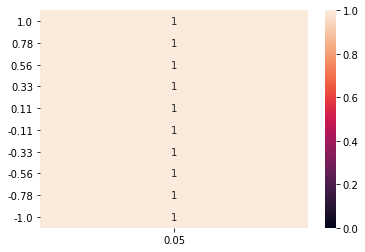
\includegraphics[width = 0.7 \textwidth]{Figures/tau_005.png}
	\caption{$\tau = 0.0$}
	\end{subfigure}
	\begin{subfigure}[b]{0.45 \textwidth}
	\centering
	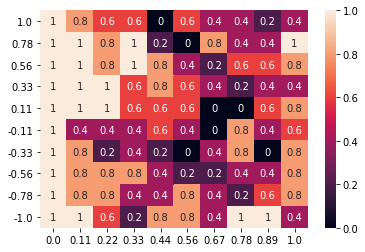
\includegraphics[width = 0.7 \textwidth]{Figures/tau_015.png}
	\caption{$\tau = 0.15$}
	\end{subfigure}

	\caption{$\alpha = 0.1$, $\gamma = 0.1$, $\tau \in [0.1, 10]$, $\Gamma \in [-1, 1]$. Each
	simulation is run for 1e5 iterations and tested for convergence. The game is said to have
	converged based on a tolerance of 1\% difference between action probabilities. For each
	combination of $\tau$, $\Gamma$ the game is played 5 times, each with random payoff matrices
	and initial conditions. The average number of converged games (giving an indication of
	probability of convergence) is shown in each cell of the heatmap. \label{fig::Toys}}
\end{figure}


To generate the numerical simulations in Figure \ref{fig::Toys} we used the following procedure.

\begin{enumerate}
	\item Fix the parameters $\alpha$ and $\gamma$. The latter is held fixed at $0.1$ since
	it does not affect the long term behaviour of the system (it does not appear in (
	\ref{eqn::EOM})).
	\item We initialise values of $\Gamma$ and $\tau$. These will be the variables which we sweep
	over.
	\item Generate payoff matrices for both agents by sampling from a multi-variate Gaussian 
	(variables are the payoff elements) with covariance parameterised by $\Gamma$.
	\item Iniitialise the agents with random initial conditions (i.e. random action probabilities).
	\item Allow the agents to learn over a maximum of $1 \times 10^5$ iterations.
	\item Every 100 iterations, check to see if the action probabilities have changed significantly.
	If not (i.e. the change over the last 100 iterations is less than 1\%) the learning is
	considered to have converged.
	\item This process is repeated 5 times with random payoff matrices generated based on the value
	of $\Gamma$. The probability of convergence is then recorded as $\frac{\text{number of times
	converged}}{5}$.
	\item The values of $\tau$ and $\Gamma$ are then modified and the process is repeated. The
	heatmap shows the probability of convergence for all values of $\tau$ and $\Gamma$ which are
	tested.
\end{enumerate}

\end{document}